\documentclass{article}
\usepackage{amsmath}
\usepackage{amssymb}
\usepackage{stmaryrd}
\usepackage{graphicx}
\usepackage{babel}
\usepackage[margin=3cm]{geometry}
\begin{document}
\title{Scanneur 3D}
\author{Ulysse DURAND}
\date{}
\maketitle

\section*{Histoire du scanner 3D}

Lors de notre projet de sciences de l'ingénieur de terminale, avec
Yann Prost, Loïc Thomas et Gabin Jobert--Rollin, nous nous sommes
lancés dans la conception d'un scanneur 3D. Nous voulions dans notre
cahier des charges pouvoir scanner un objet opaque et rigide pouvant
rentrer dans un cylindre de 20cm de rayon et de 20cm de hauteur pour
fournir un fichier 3D dans un format .obj représentant l'objet. Aprés
plusieurs idées irréalisables comme utiliser un palpeur sur 3 axes
de translation, et un axe de rotation pour l'objet, nous nous sommes
résiliés au concept de 'capture d'ombre'.

Le résultat est alors assez satisfaisant pour 'cloner' les objets
scannés, à l'aide d'une imprimante 3D.

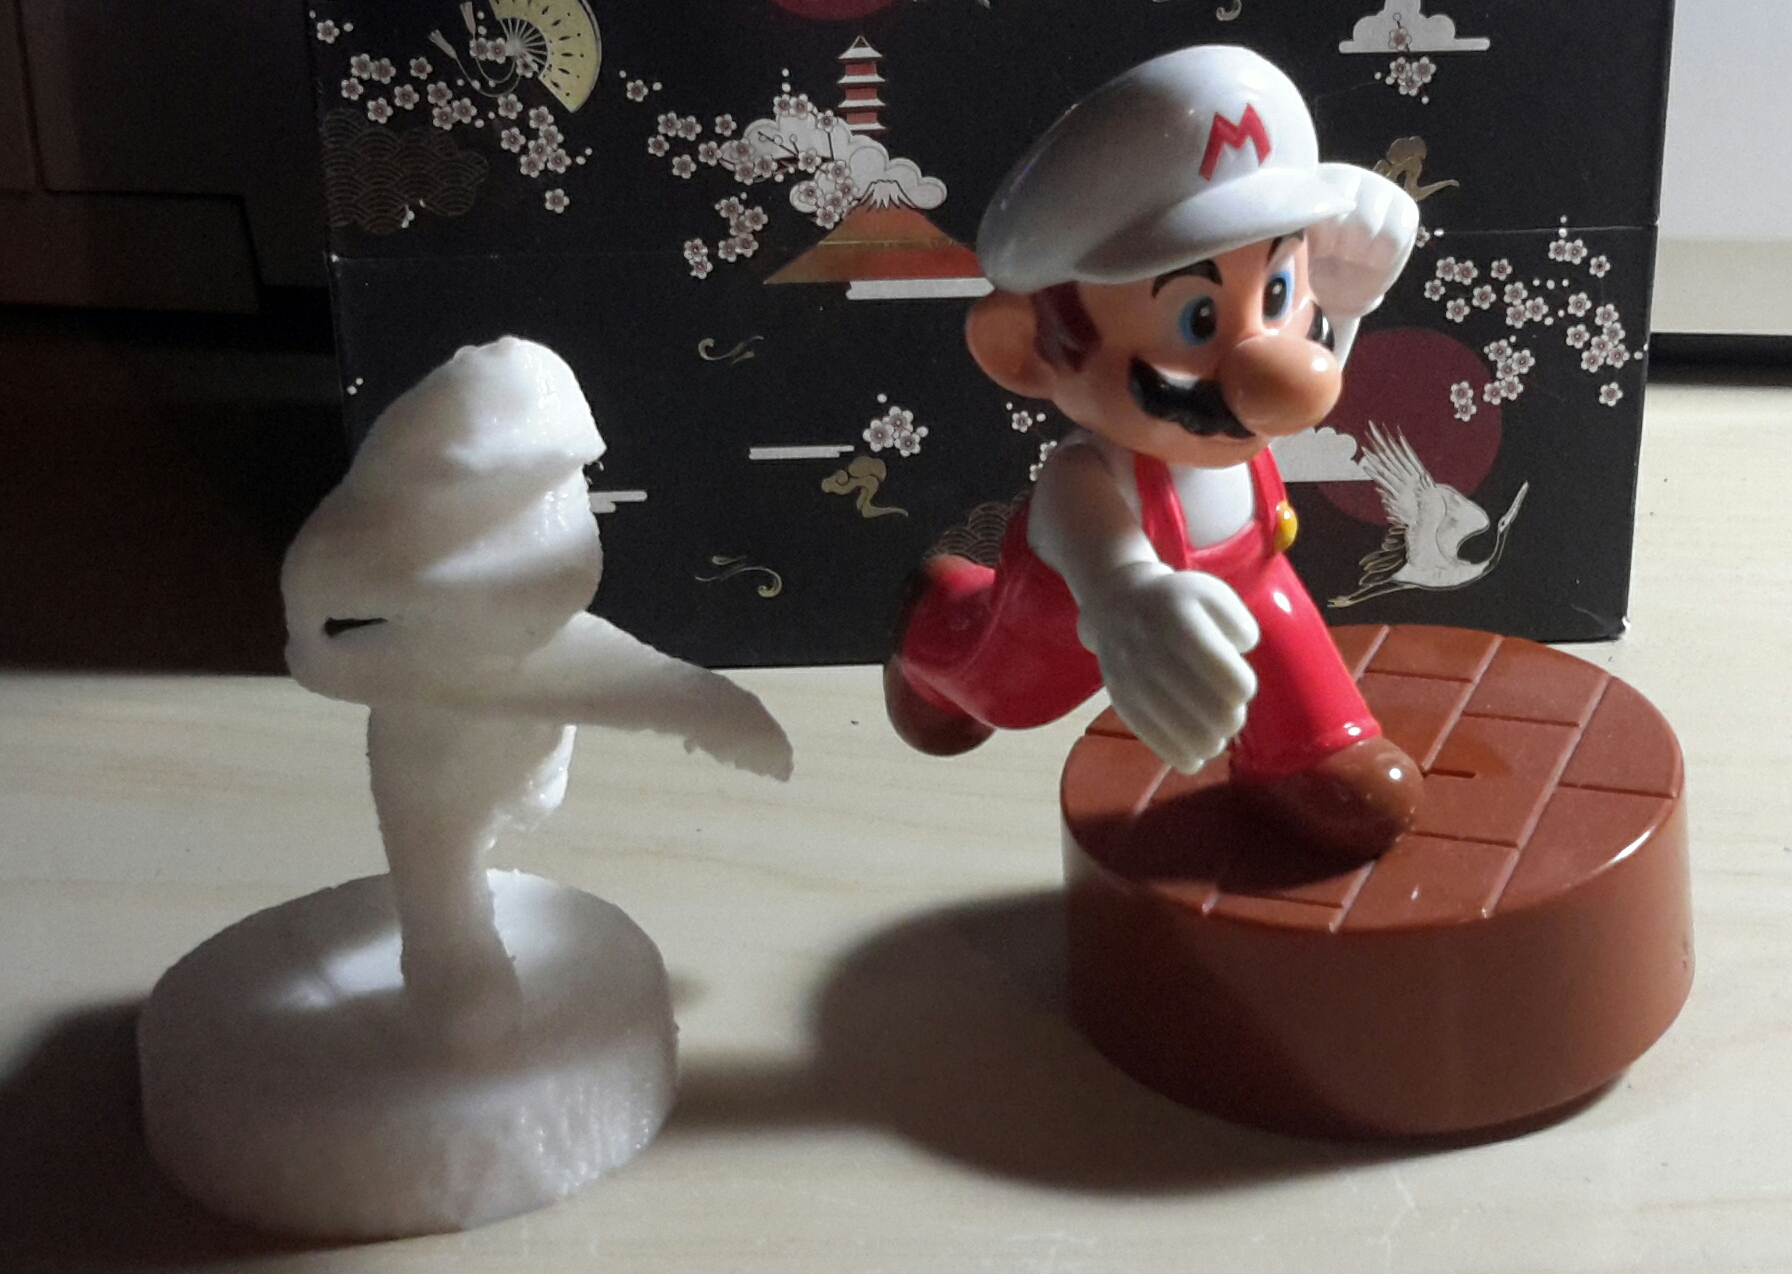
\includegraphics[scale=0.1]{10}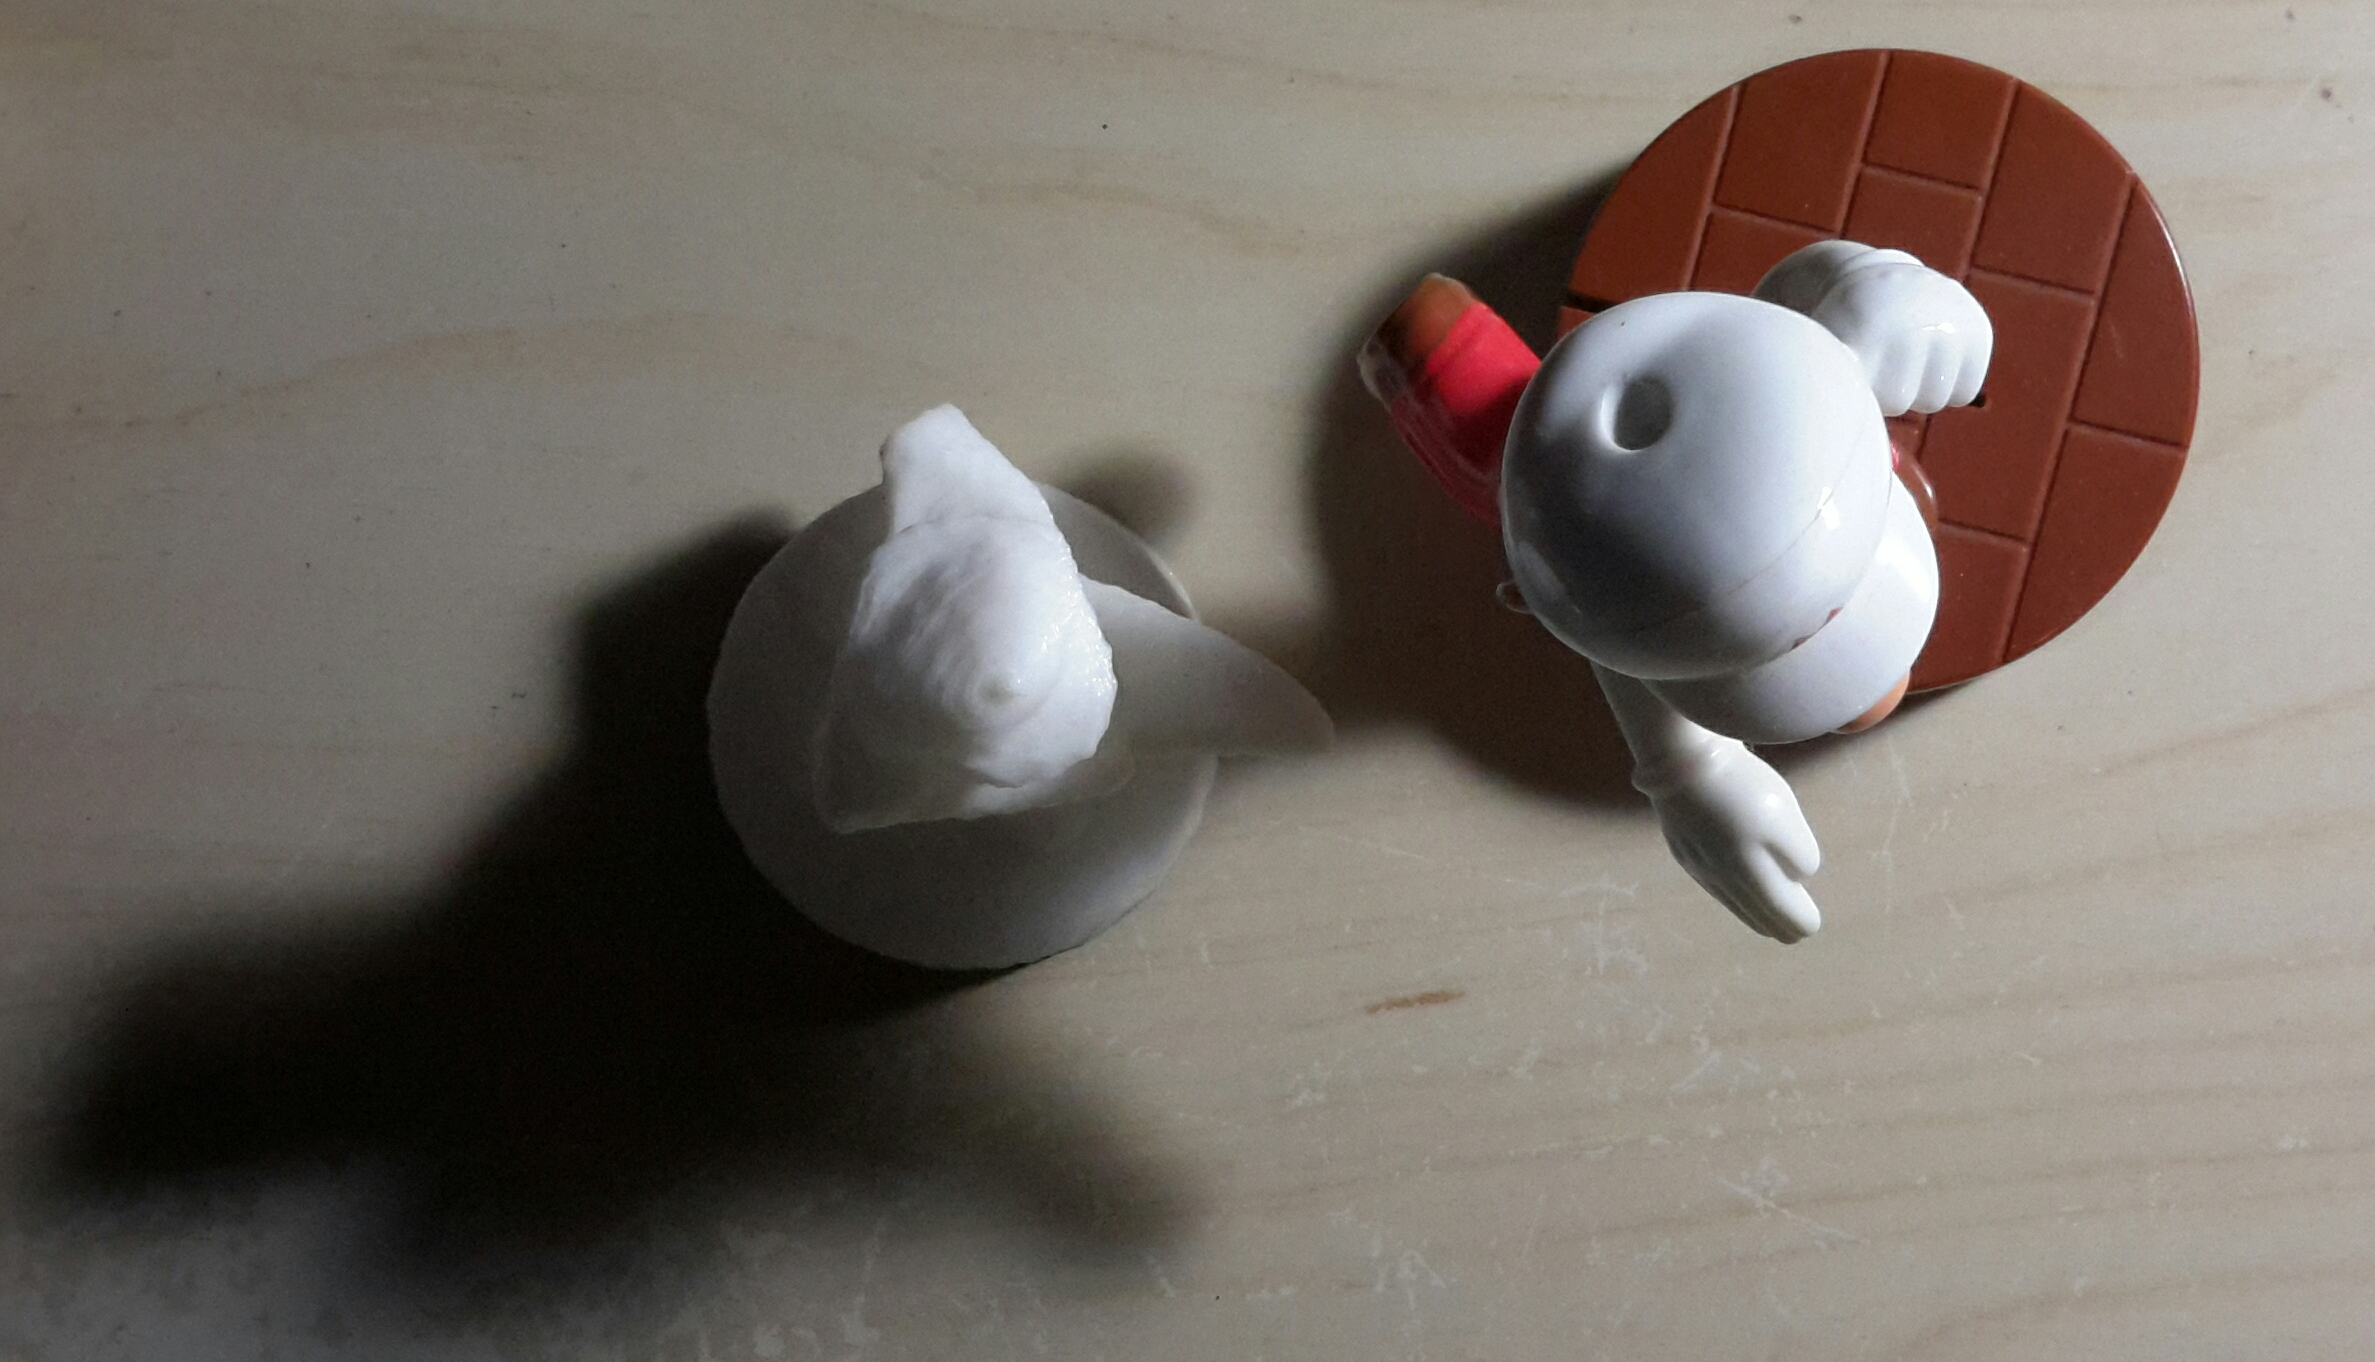
\includegraphics[scale=0.1]{11}

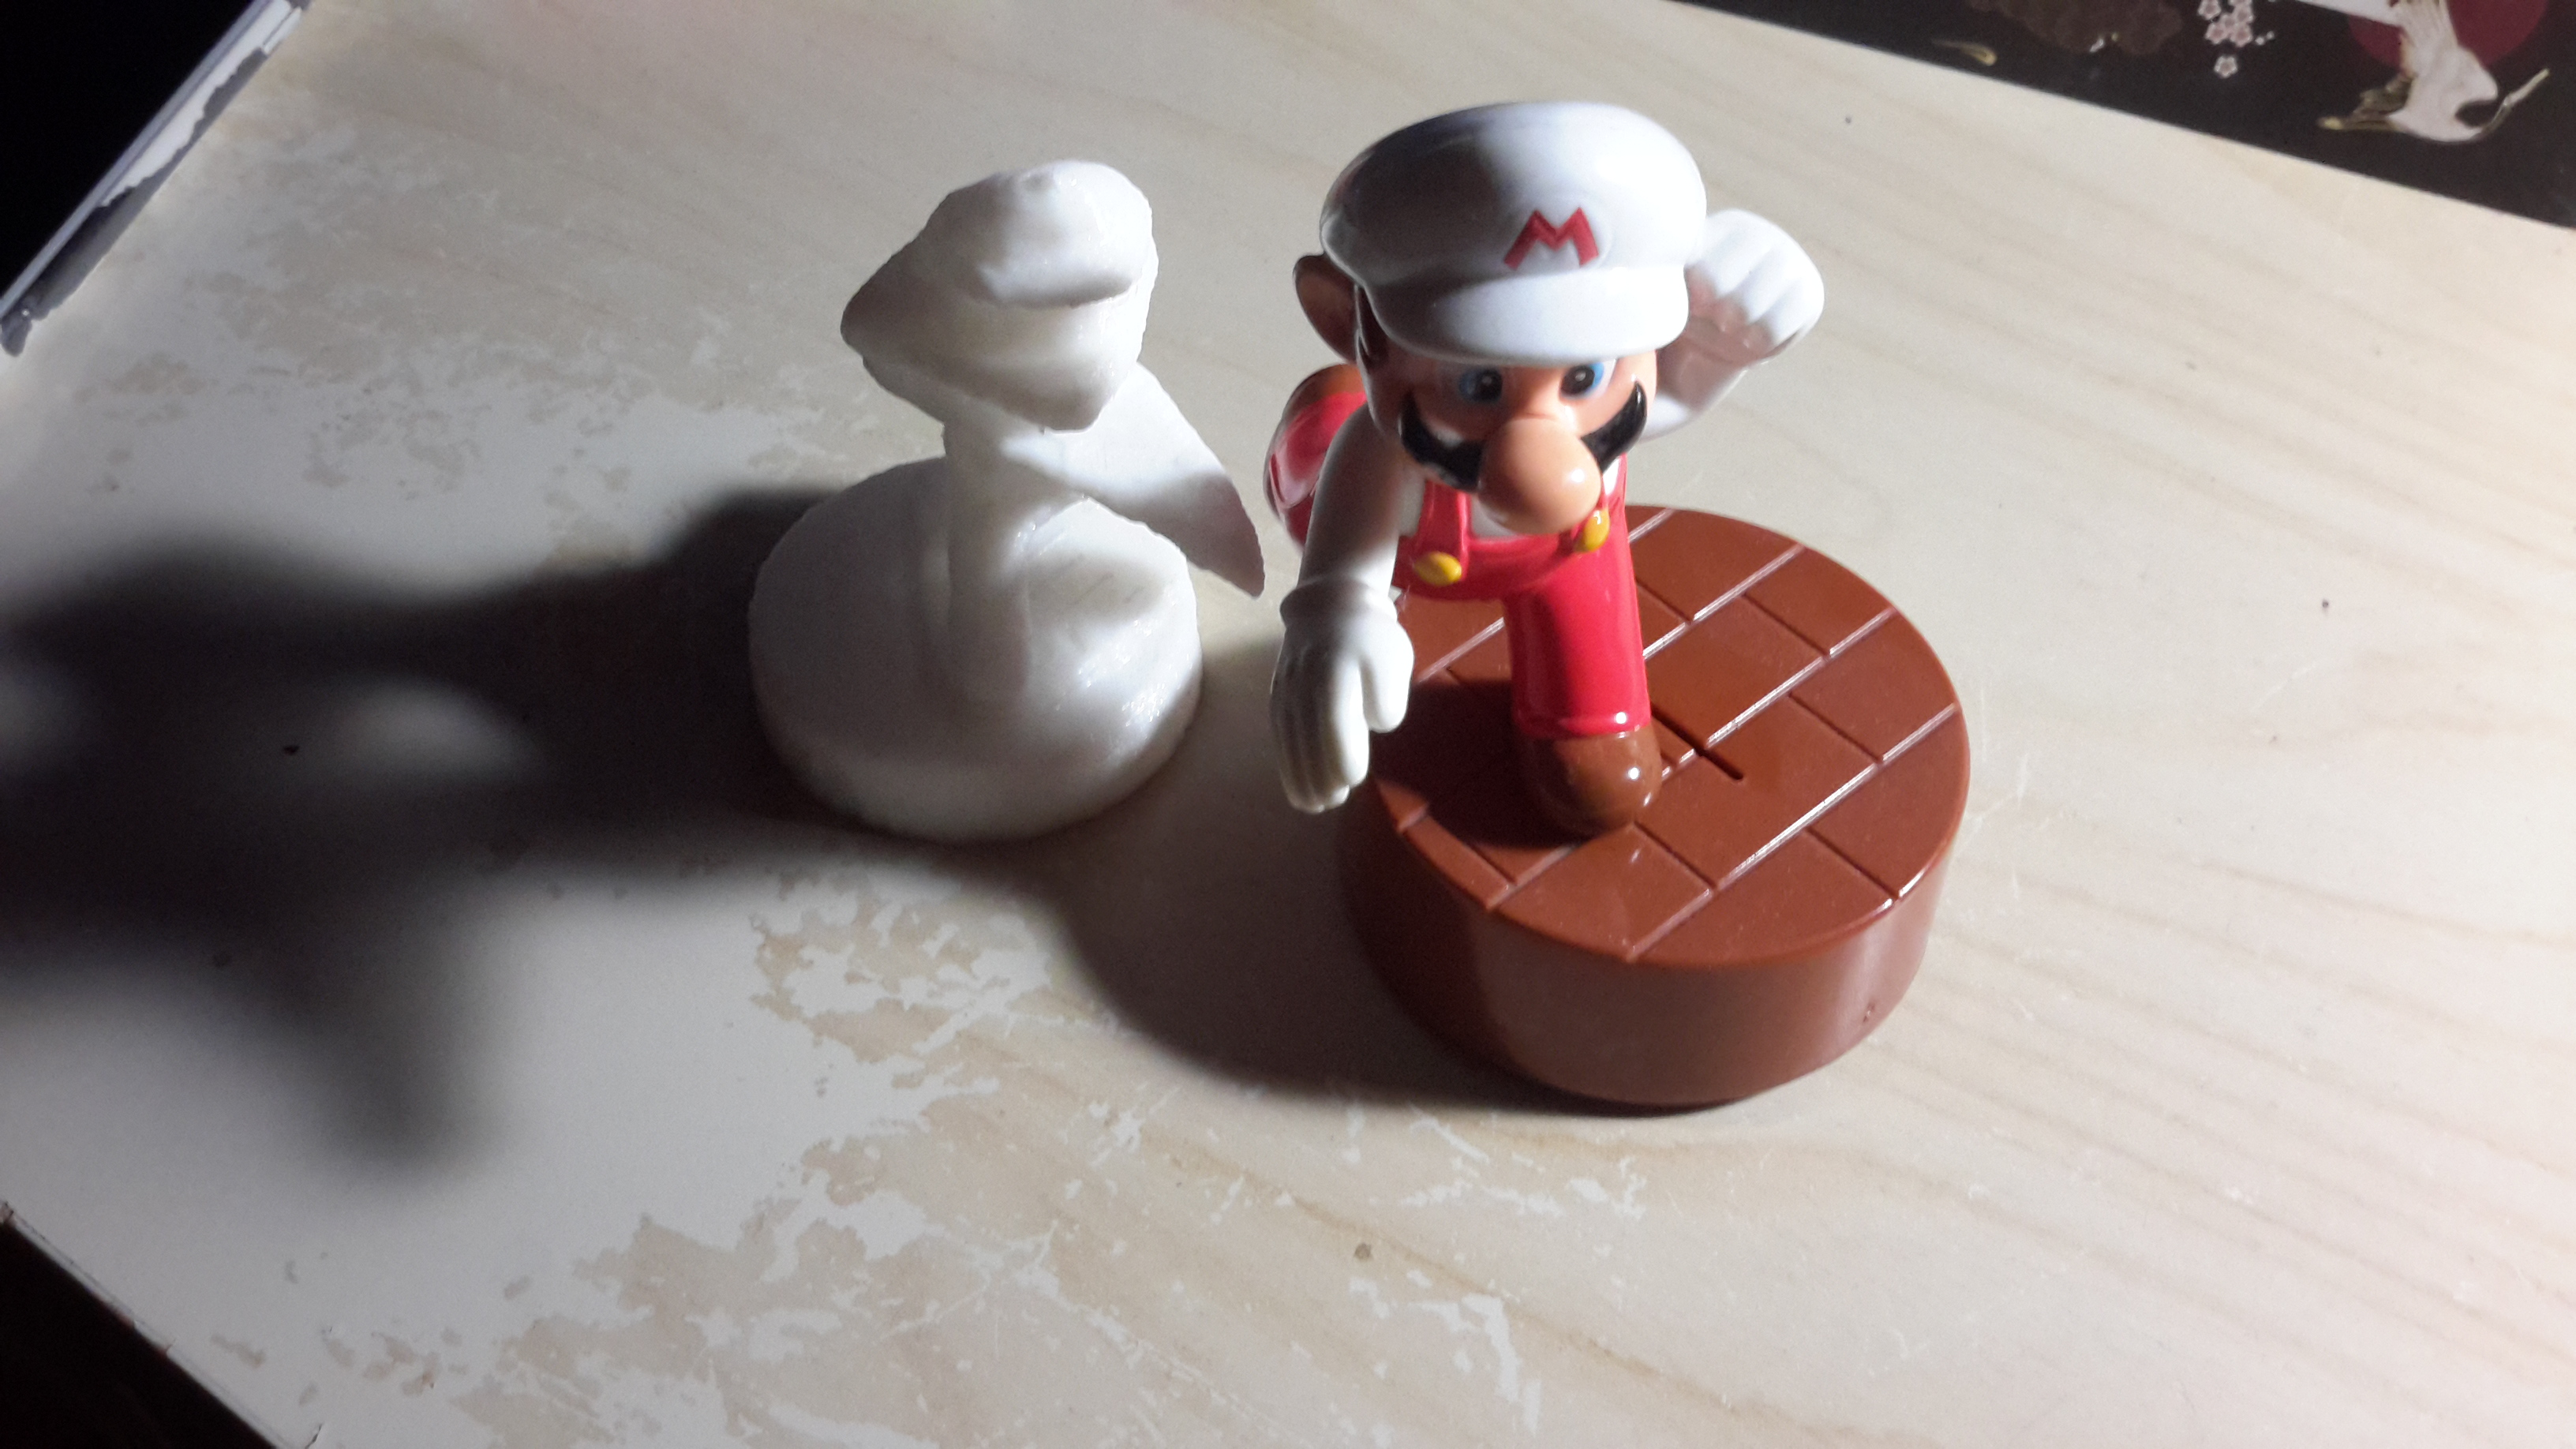
\includegraphics[scale=0.1]{12}

\subsubsection*{La capture d'ombre :}

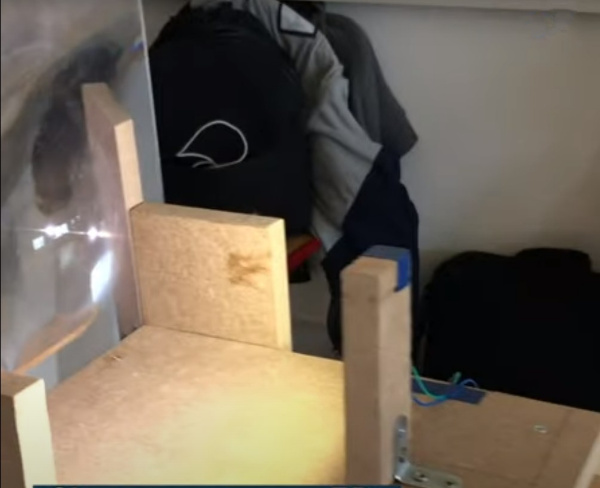
\includegraphics[scale=0.25]{1}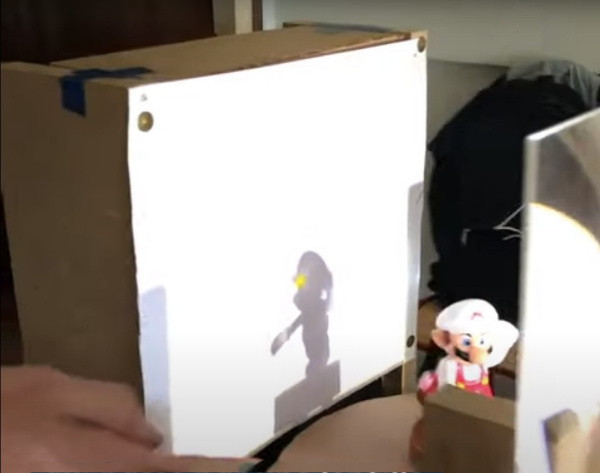
\includegraphics[scale=0.25]{2}

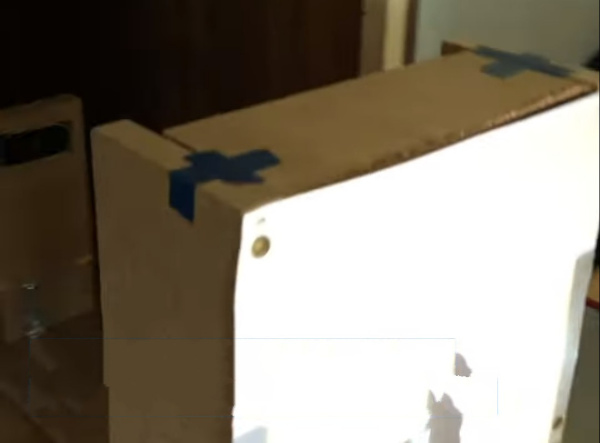
\includegraphics[scale=0.25]{3}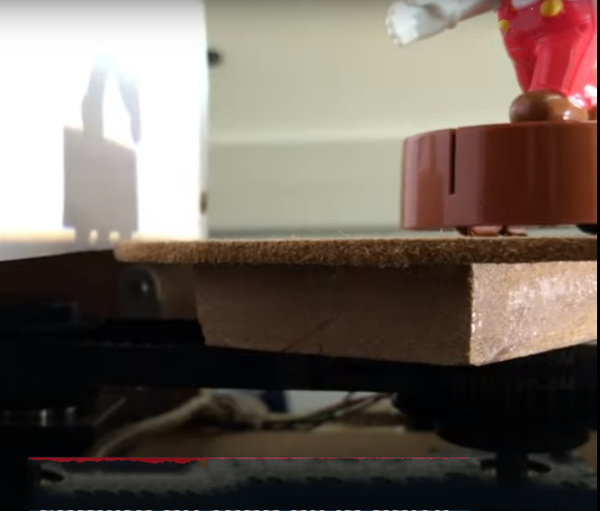
\includegraphics[scale=0.25]{4}

L'objet à scanner est placé dans une boite noire sur un plateau tournant,
il est éclairé par une lumière dont les rayons sont parallèles et
l'ombre de l'objet est projetée sur un écran semi transparent (feuille
de papier). Ainsi de l'autre côté de l'écran, une caméra peut prendre
l'ombre de l'objet en photo, entre chaque photo, l'objet tourne légèrement
autour d'un axe vertical. On se retrouve avec une liste de photos
de l'ombre de l'objet pris sous différents angles. Et avec ces ombres
le but est de reconstituer l'objet en 3D.

Les solutions techniques sont les suivantes, pour avoir des rayons
lumineux parallèles, on a utilisé une lentille de Fresnel qui agit
comme une grande lentille convergente, avec une LED en son foyer.
On a fait pivoter l'objet grâce à un plateau tournant (sur un roulement
à billes) lié à un moteur pas à pas par une courroi de transmission.
Le moteur pas à pas étant controlé par un arduino qui communique en
série avec le logiciel sur ordinateur. La caméra est connectée comme
webcam à l'ordinateur pour prendre les photos quand le logiciel en
a besoin.

La conception materielle du scanneur et le logiciel d'acquisition
(qui prend des photos et controle le moteur) ont été respectivement
développés par Yann Prost et Loïc Thomas.

\subsubsection*{Le traitement des données :}

Enfin, nous avions notre liste d'images.

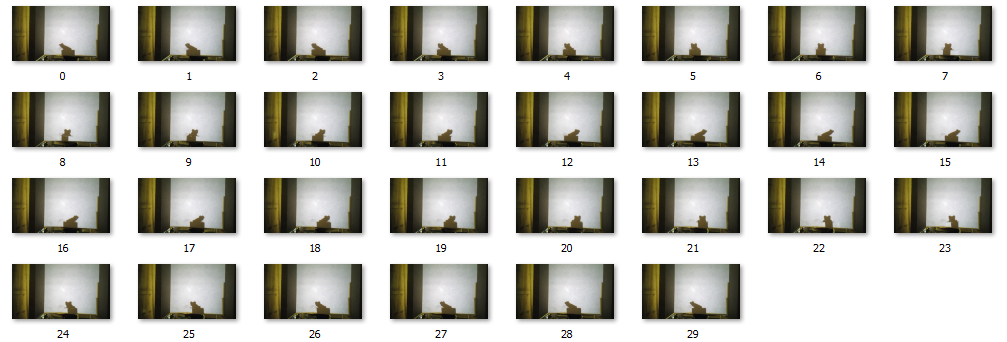
\includegraphics[scale=0.25]{5}

Une première étape était de faire un premier traitement des images
qui détermine si à un certain endroit de l'écran on est ou pas dans
l'ombre de l'objet. C'est Gabin Jobert--Rollin qui s'en est occupé.

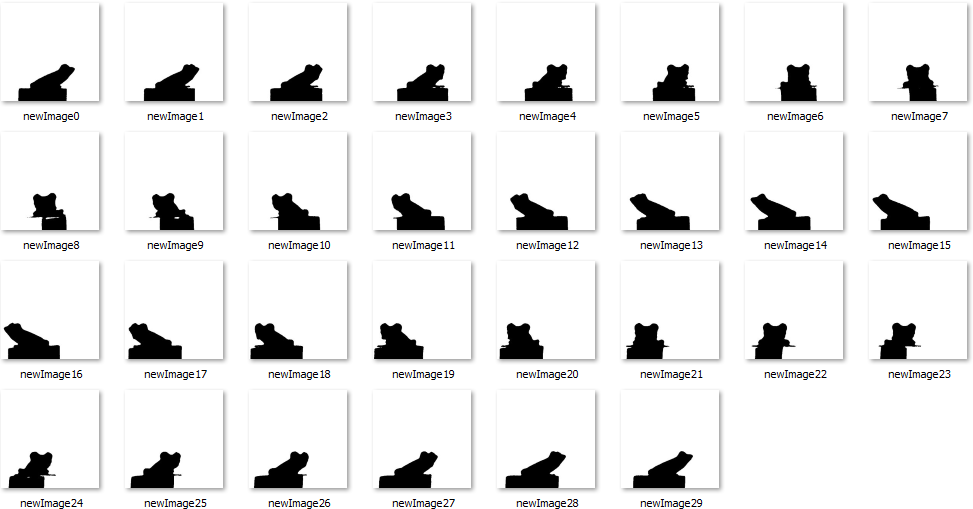
\includegraphics[scale=0.25]{6}

Je devais alors personnellement m'occuper de faire ce dernier traitement
qui à partir d'une image en noir ou blanc de l'ombre de l'objet génère 
le fichier .obj.

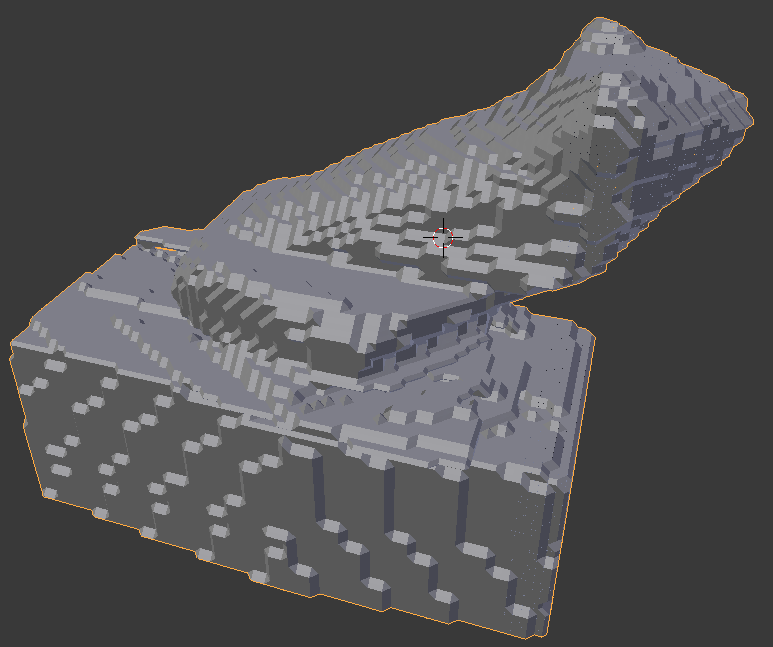
\includegraphics[scale=0.25]{9}

\section*{La génération du fichier 3D}

\subsection*{Première approche relativement simple.}

Notations : 
\begin{itemize}
    \item $\mathcal{S}\in\mathcal{P}(\mathbb{R}^{3})$ sera une approximation
          de l'objet que l'on veut modéliser.
    \item $res\in\mathbb{N}$sera un paramètre de résolution, plus il est grand
          plus le résultat sera proche de $\mathcal{S}$.
    \item $P_{\theta}=\{(x,y,z)\in\mathbb{R}^{3}|\frac{y}{x}=\tan(\theta)\}$
          est le plan qui passe par l'origine et qui a un angle $\theta$ avec
          le plan $xOz$. On associe à chaque plan $P_{\theta}$une base orthonormée
          $B_{\theta}=(0,\overrightarrow{u_{\theta}},\overrightarrow{v_{\theta}})$
          avec $\overrightarrow{u_{\theta}}=(\cos\theta,\sin\theta,0)$ et $\overrightarrow{v_{\theta}}=(-\sin\theta,\cos\theta,0)$.
    \item $f_{\theta}=\left(\begin{array}{c}
                      \mathbb{R}^{2}\longrightarrow\{0,1\} \\
                      (x,y)\mapsto\begin{cases}
                          1 & \text{si il y a de l'ombre aux coordonnées \ensuremath{(x,y)} de l'image \ensuremath{\theta}} \\
                          0 & \text{sinon}
                      \end{cases}
                  \end{array}\right)$
    \item la projection $p(M,P):\mathbb{R}^{3}\times\mathcal{P}\longrightarrow\mathbb{R}^{2}$
          ($\mathcal{P}$ est l'ensemble des plans de $\mathbb{R}^{3}$) au
          point M et au plan P associe les coordonnées de la projection orthogonale
          de M sur le plan P dans la base de ce plan.
\end{itemize}
Première idée qui est très couteuse en calcul mais fonctionnelle,
on a un ensemble de points dans l'espace $\mathcal{E}=\{-\frac{1}{2}+\frac{k}{res}|k\in\llbracket0,res\llbracket\}^{3}\in\mathcal{P}(\mathbb{R}^{3})$
et on regarde si ces points appartiennent à $\mathcal{S}$, 

soit $\forall M\in\mathcal{E},M\in\mathcal{S}\Leftrightarrow\forall\theta\in\{0,\frac{\pi}{n},2\frac{\pi}{n},...,(n-1)\frac{\pi}{n}\},f_{\theta}(p(M,P_{\theta}))=1$.

Alors avec cette caracterisation on obtient $\mathcal{E}\cap\mathcal{S}$.
et avec, on peut passer à la prochaine étape, la création du fichier
.obj.

\subsubsection*{Création du fichier .obj à partir de $\mathcal{E}\cap\mathcal{S}$.}

Un fichier obj, de quoi c'est constitué ? C'est un fichier contenant
une liste de sommets, puis une liste de faces triangles (3 indices
de sommets) orientée (sommets ordonnés pour la règle du tir bouchon)

Pour créer ce fichier obj, on utilise l'algorithme marching cubes
.\cite{key-1}

Mais alors, le résultat de marching cube sera lui une approximation de $\mathcal{S}$,
pas le meilleur résultat possible et en plus, il nécessite beaucoup
de calculs (complexité en $\mathcal{O}(res^{3})$)

\subsection*{Deuxième approche plus précise et rapide}

dans cette deuxième approche, on va tout traiter par intersection
de polygones.

Remarque : on peut traiter indépendamment les lignes de pixels des
images.

pour un z donné, on a une ligne de pixels pour chaque angle, ligne
qu'on peut décomposer en segments. ex : 10010111101100100 peut se
décomposer en : S(0,1),S(3,4),S(5,9),S(10,12),S(14,15).

On note alors l'ensemble des décompositions pour la ligne z de l'image
$\theta$ $d_{z,\theta}$. On peut par exemple avoir $d_{0.34,\frac{35\pi}{180}}=\{S(-0.87,-0.22),S(-0.02,0.65)\}$.

Ensuite, pour chaque segment de décomposition on construit un quadrilatere,
de largeur celle du segment en question et de longueur infinie qui
a $\theta$ pour angle avec l'axe x, et c'est en faisant l'intersection
des polygones de toutes les decompositions pour un z donné qu'on aura
une coupe de $\mathcal{S}$selon le plan de hauteur z.

Un petit exemple : 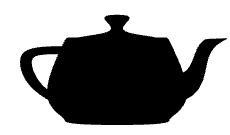
\includegraphics[scale=0.5]{14}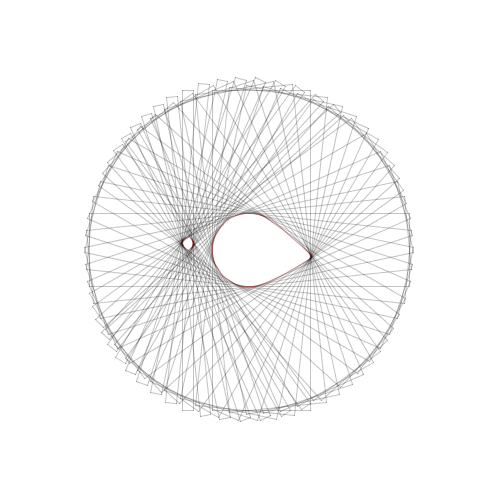
\includegraphics[scale=0.25]{13}

Pour ce qui est de l'intersection ou l'union de polygones, on considère
la surface délimitée par leur bords.

Il faut alors passer d'intersection d'union de polygones à union d'intersection
de polygones, en utilisant le fait que $\bigcap_{i\in I}\bigcup_{j\in J_{i}}A_{i,j}=\bigcup_{f\in(\prod_{i\in I}J_{i})}\bigcap_{i\in I}A_{i,f(i)}$.

pour faire des intersections de polygones, on utilise l'algorithme
de O'Rourke \cite{key-1} qui permet de faire l'intersection de deux
polygones convexes de respectivement m et n côtés en une complexité
en $\mathcal{O}(n+m)$.

\subparagraph{Création du fichier .obj à partir des coupes de S}

On veut relier les différentes coupes entre elles pour en faire un
fichier .obj, donc faire une surface triangularisée.
\begin{thebibliography}{1}
    \bibitem{key-1}William E. Lorensen et Harvey E.Cline. Marching Cubes:
    A High Resolution 3D Surface Construction Algorithm (août 1987).
    
    \bibitem{key-1}Joseph O\textquoteright Rourke, Chi-Bin Chien, Thomas
    Olson, and David Naddor. A New Linear Algorithm for Intersecting Convex
    Polygons (7/10/1981)
\end{thebibliography}

\end{document}
